% Auto-generated by leakage_emergence.plotting.generate_all_figures.
% These captions describe finite-dimensional numerical illustrations;
% they do not claim to prove the infinite-dimensional theorem statements.

% 01_component_norms.pdf
% Supports: The first-order emergence theorem, by showing observable-sector growth from hidden initial data when the leakage block is active.
\begin{figure}[t]
  \centering
  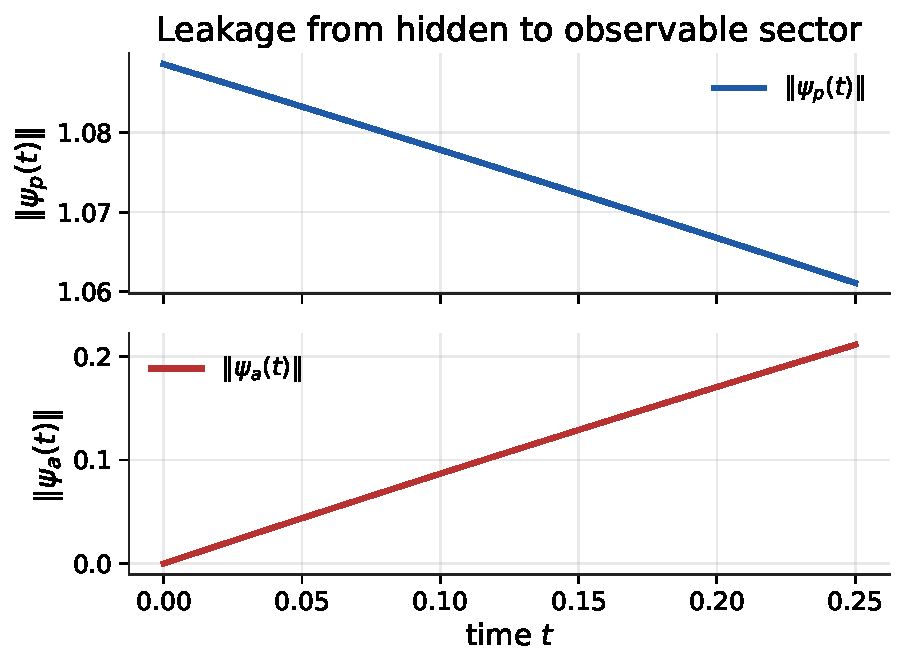
\includegraphics[width=0.82\linewidth]{figures/01_component_norms.pdf}
  \caption{Finite-dimensional illustration of leakage from the hidden sector to the observable sector. The upper panel shows the hidden component norm $\|\psi_p(t)\|$, while the lower panel shows the observable component norm $\|\psi_a(t)\|$ generated by a nonzero leakage block. \emph{Theorem support:} The first-order emergence theorem, by showing observable-sector growth from hidden initial data when the leakage block is active.}
  \label{fig:leakage-norms}
\end{figure}

% 02_first_order_emergence.pdf
% Supports: The first-order emergence statement.
\begin{figure}[t]
  \centering
  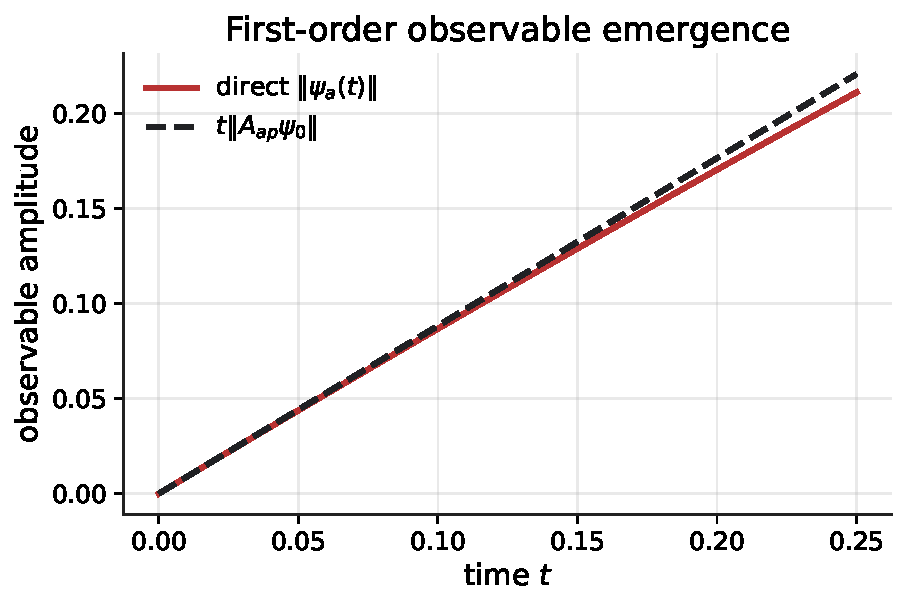
\includegraphics[width=0.82\linewidth]{figures/02_first_order_emergence.pdf}
  \caption{Comparison of the directly computed observable amplitude $\|\psi_a(t)\|$ with the leading term $t\|A_{ap}\psi_0\|$ for a hidden initial state. Agreement at early times illustrates the finite-dimensional version of $\psi_a(t)=tA_{ap}\psi_0+o(t)$. \emph{Theorem support:} The first-order emergence statement.}
  \label{fig:first-order-emergence}
\end{figure}

% 03_duhamel_agreement.pdf
% Supports: The integrated leakage identity.
\begin{figure}[t]
  \centering
  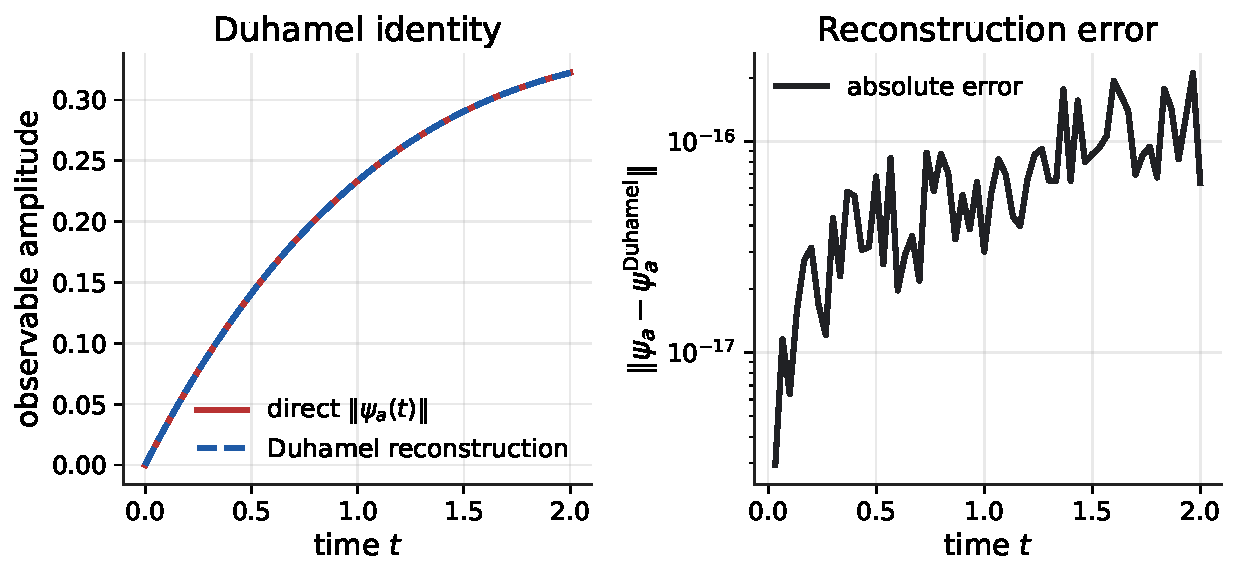
\includegraphics[width=0.82\linewidth]{figures/03_duhamel_agreement.pdf}
  \caption{Direct observable-sector evolution compared with the Duhamel variation-of-constants reconstruction. The error panel reports the norm of the difference between the two finite-dimensional computations. \emph{Theorem support:} The integrated leakage identity.}
  \label{fig:duhamel-agreement}
\end{figure}

% 04_threshold_crossing.pdf
% Supports: The thresholded-observation construction.
\begin{figure}[t]
  \centering
  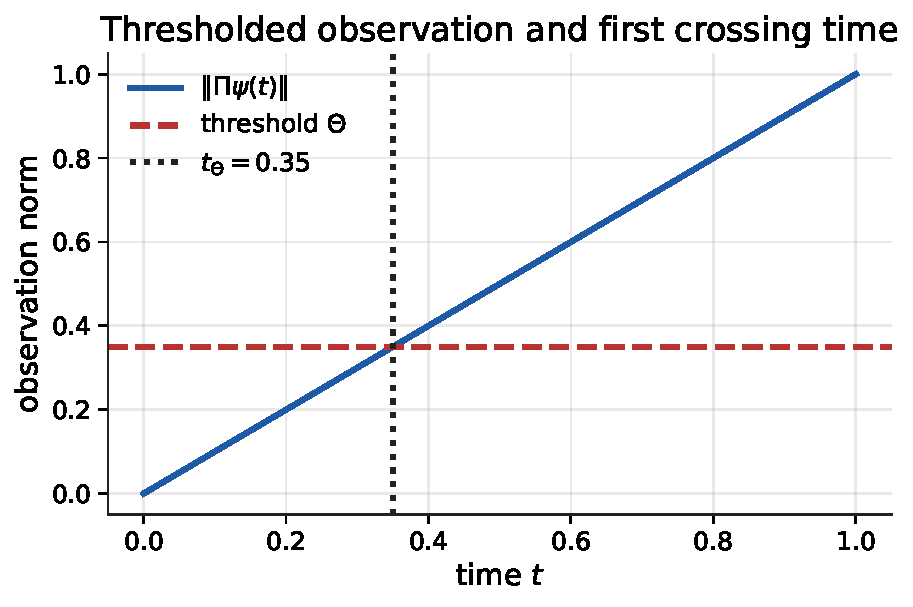
\includegraphics[width=0.82\linewidth]{figures/04_threshold_crossing.pdf}
  \caption{Thresholded observation for the awareness signal $\|\Pi\psi(t)\|$. The horizontal line marks the threshold $\Theta$, and the vertical line marks the interpolated first crossing time $t_\Theta$. \emph{Theorem support:} The thresholded-observation construction.}
  \label{fig:threshold-crossing}
\end{figure}

% 05_spectral_hiddenness.pdf
% Supports: The spectral hiddenness criterion.
\begin{figure}[t]
  \centering
  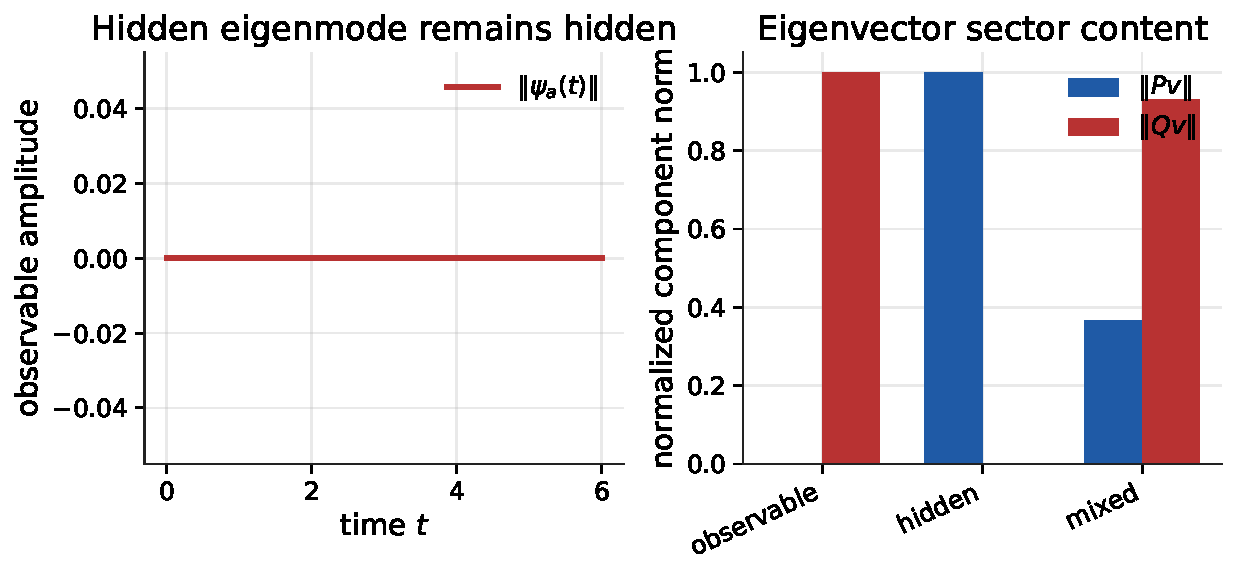
\includegraphics[width=0.82\linewidth]{figures/05_spectral_hiddenness.pdf}
  \caption{Hidden eigenmode example. A hidden eigenvector remains in the hidden sector under the flow, while the bar plot reports the hidden and observable content of eigenvectors in the finite-dimensional operator. \emph{Theorem support:} The spectral hiddenness criterion.}
  \label{fig:spectral-hiddenness}
\end{figure}

% 06_resolvent_leakage.pdf
% Supports: The resolvent leakage criterion.
\begin{figure}[t]
  \centering
  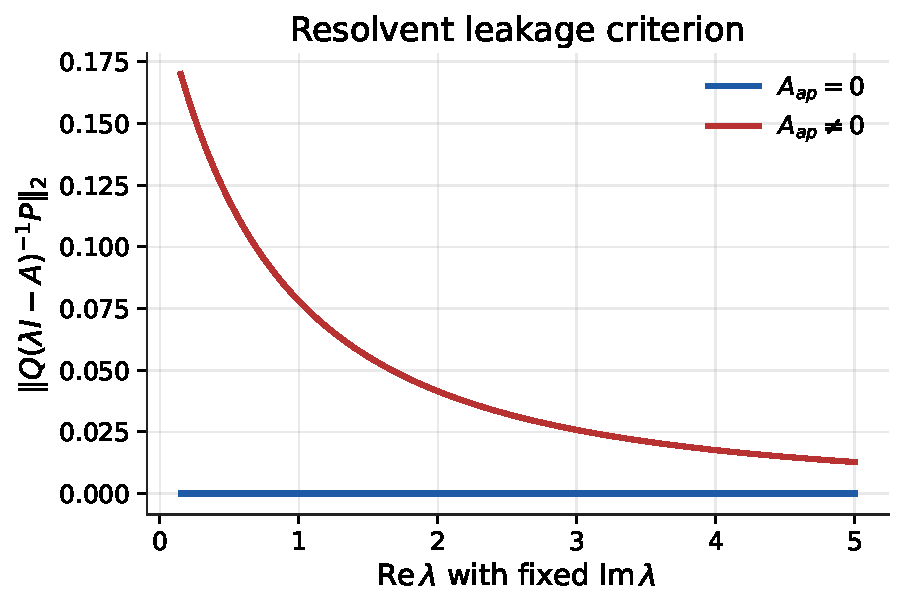
\includegraphics[width=0.82\linewidth]{figures/06_resolvent_leakage.pdf}
  \caption{Leakage-resolvent norm $\|Q(\lambda I-A)^{-1}P\|_2$ along a complex line in the resolvent set. The invariant example has zero leakage norm, while the leaky example produces nonzero hidden-to-observable mixing through the resolvent. \emph{Theorem support:} The resolvent leakage criterion.}
  \label{fig:resolvent-leakage}
\end{figure}

% 07_nonlinear_emergence.pdf
% Supports: The nonlinear invariance and nonlinear emergence examples.
\begin{figure}[t]
  \centering
  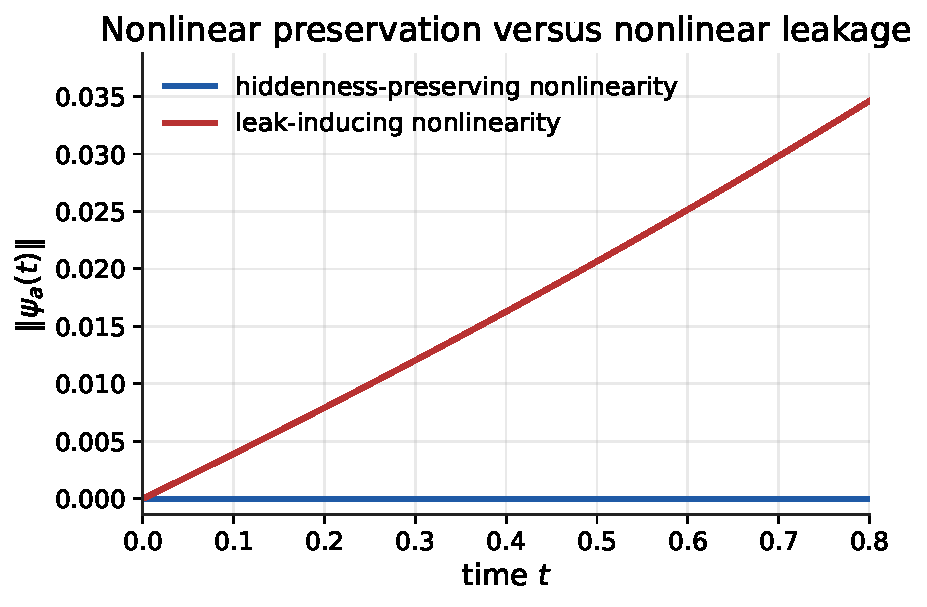
\includegraphics[width=0.82\linewidth]{figures/07_nonlinear_emergence.pdf}
  \caption{Nonlinear hiddenness preservation versus nonlinear leakage. The sector-preserving cubic example keeps the observable norm at zero, whereas the rotated hidden sector with the same elementwise cubic mechanism develops an observable component. \emph{Theorem support:} The nonlinear invariance and nonlinear emergence examples.}
  \label{fig:nonlinear-leakage}
\end{figure}

% 08_early_time_scaling.pdf
% Supports: The second-order energy emergence diagnostic.
\begin{figure}[t]
  \centering
  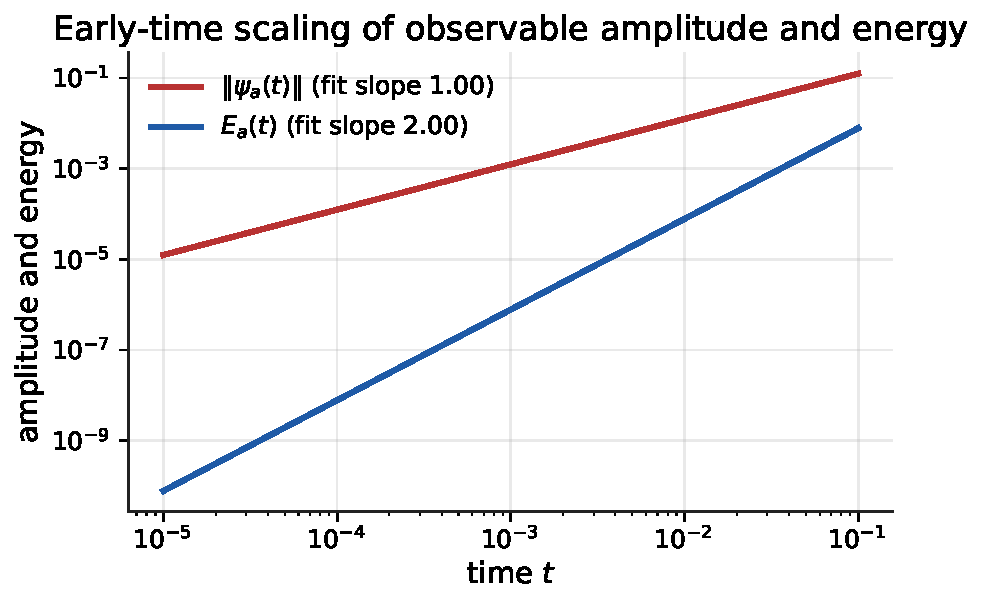
\includegraphics[width=0.82\linewidth]{figures/08_early_time_scaling.pdf}
  \caption{Log--log early-time scaling of observable amplitude and aware-sector energy. The fitted slopes show $\|\psi_a(t)\|=O(t)$ and $E_a(t)=O(t^2)$ in this finite-dimensional leakage-active example. \emph{Theorem support:} The second-order energy emergence diagnostic.}
  \label{fig:early-time-scaling}
\end{figure}
